\documentclass{standalone}
%\usepackage{tikz}
%\usetikzlibrary{arrows.meta}
\usepackage{pgfplots}
\pgfplotsset{compat = newest}
%\tikzset{>=Latex}
\usepackage{tikz}
\usetikzlibrary{arrows.meta}
\tikzset{label/.style = {inner sep=1pt, fill=white}}
%\tikzset{nd/.style={circle, inner sep=0pt}}
\tikzset{nd/.style={inner sep=1pt}}
\tikzset{>=Latex}
\tikzset{arc/.style = {->, semithick, >=Latex}}
\begin{document}
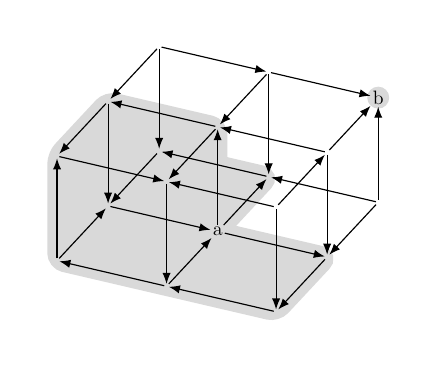
\begin{tikzpicture}[scale=.7]
\begin{axis}[
    axis line style = {color=white},
    %xlabel={$P_1$},
    %ylabel={$P_2$},
    %zlabel={$P_3$},
    xmin=-1.1, xmax=1.1,
    ymin=-1.1, ymax=1.1,
    zmin=-0.1, zmax=1.1,
    axis equal image,
    %ticks =none,
    %xtick = 0,
    xticklabels = {},
    %ytick = {0,1},
    yticklabels = {},
    %ztick = {0,1},
    zticklabels = {},
    xtick style = {draw=none},
    ytick style = {draw=none},
    ztick style = {draw=none},
]

    %\draw [rounded corners, color = gray!30, line width = 10pt] (1,0,1) to (0,0,1) to (0,1,1) to (0,1,0) to (1,1,0) to (1,0,0) -- cycle;

    %\draw [rounded corners, color = gray!30, line width = 10pt, fill] (0,0,0) to (1,0,0) to (1,-1,0) to (0,-1,0) to (-1,-1,0) to (-1,-1,1) -- (-1,0,1) -- (0,0,1) -- (0,0,0) -- (0,1,0) -- (-1,1,0) -- (-1,0,0) -- cycle;

    \draw [rounded corners, color = white, line width = 10pt, fill] (-1.1,-1.1,-0.1) to (-1.1,-1.1,1.1) to (-1.1,1.1,1.1) to (1.1,1.1,1.1) to (1.1,1.1,0.1) to (1.1,-1.1,0.1) to cycle;

    \draw [rounded corners, color = gray!30, line width = 10pt, fill] (0,0,0) to (1,0,0) to (1,-1,0) to (0,-1,0) to (-1,-1,0) to (-1,-1,1) -- (-1,0,1) -- (0,0,1) -- (0,0,0) -- (0,1,0) -- (-.4,1,0);

    \node[nd,color = gray!30, circle, inner sep= 4pt, fill] at (1,1,1) {};

    %\node (H1) at (-2,0) {$H$:};
    %\node (T1) at (-0.8,1) {$T$:};
    
    \node[nd] (hhh) at (0,0,0) {a};
    \node[nd] (thh) at (1,0,0) {};
    \node[nd] (hht) at (0,0,1) {};
    \node[nd] (tht) at (1,0,1) {};
    
    \node[nd] (hth) at (0,1,0) {};
    \node[nd] (tth) at (1,1,0) {};
    \node[nd] (htt) at (0,1,1) {};
    \node[nd] (ttt) at (1,1,1) {b};

    \node[nd] (a) at (-1,0,0) {};
    \node[nd] (b) at (-1,0,1) {};
    \node[nd] (c) at (-1,1,0) {};
    \node[nd] (d) at (-1,1,1) {};
    
    \node[nd] (e) at (0,-1,0) {};
    \node[nd] (f) at (0,-1,1) {};
    \node[nd] (g) at (1,-1,0) {};
    \node[nd] (h) at (1,-1,1) {};

    \node[nd] (i) at (-1,-1,0) {};
    \node[nd] (j) at (-1,-1,1) {};
    
    %\node (o) at (-2.5,-1) {$H$};
    %\node (z) at (-1,-0.2) {$T$};
    %\node (x) at (-0.9,-1) {$T$};
    %\node (y) at (-2.5,0.5) {$T$};
    %\draw (o) -- node[above] {$P_2$} (z);
    %\draw (o) -- node[below] {$P_1$} (x);
    %\draw (o) -- node[left] {$P_3$} (y);
    
    \draw[arc] (hhh) to (hht);
    \draw[arc] (hhh) to (hth);
    \draw[arc] (hhh) to (thh);
    \draw[arc] (htt) to (ttt);
    \draw[arc] (tth) to (ttt);
    \draw[arc] (tht) to (ttt);
    \draw[arc] (htt) to (hht);
    \draw[arc] (tht) to (hht);
    \draw[arc] (htt) to (hth);
    \draw[arc] (tth) to (hth);
    \draw[arc] (tth) to (thh);
    \draw[arc] (tht) to (thh);

    \draw[arc] (h) to (tht);
    \draw[arc] (d) to (htt);
    \draw[arc] (thh) to (g);
    \draw[arc] (g) to (e);
    \draw[arc] (hth) to (c);
    \draw[arc] (c) to (a);
    \draw[arc] (h) to (g);
    \draw[arc] (h) to (f);
    \draw[arc] (d) to (b);
    \draw[arc] (d) to (c);
    \draw[arc] (hht) to (b);
    \draw[arc] (hht) to (f);
    \draw[arc] (f) to (e);
    \draw[arc] (b) to (a);
    \draw[arc] (e) to (hhh);
    \draw[arc] (a) to (hhh);
    \draw[arc] (b) to (j);
    \draw[arc] (j) to (f);
    \draw[arc] (e) to (i);
    \draw[arc] (i) to (a);
    \draw[arc] (i) to (j);
\end{axis}
 \end{tikzpicture}
\end{document}